%\documentclass{beamer}
%\usetheme{Pittsburgh}
\documentclass{scrartcl}

\usepackage[utf8]{inputenc}
\usepackage{default}
\usepackage[procnames]{listings}
\usepackage{graphicx}
%\usepackage[toc,page]{appendix}
\usepackage{caption}
\usepackage{hyperref}
\usepackage{color}
\usepackage{csvsimple}
\usepackage{float}
\usepackage[T1]{fontenc}



%Bibliogrpahy?
%\usepackage{bibentry}
%\nobibliography*
%\bibentry{ }


%Java
\definecolor{javared}{rgb}{0.6,0,0} % for strings
\definecolor{javagreen}{rgb}{0.25,0.5,0.35} % comments
\definecolor{javapurple}{rgb}{0.5,0,0.35} % keywords
\definecolor{javadocblue}{rgb}{0.25,0.35,0.75} % javadoc
\lstset{language=Java,
    basicstyle=\ttfamily,
    keywordstyle=\color{javapurple}\bfseries,
    stringstyle=\color{javared},
    commentstyle=\color{javagreen},
    morecomment=[s][\color{javadocblue}]{/**}{*/},
    breaklines = true,
    columns=fullflexible,
    %Numbering and tabs
    %numbers=left,
    %numberstyle=\tiny\color{gray},
    %stepnumber=2,
    %numbersep=1em,
    tabsize=4,
    showspaces=false,
    showstringspaces=false}

%Python
\definecolor{keywords}{RGB}{255,0,90}
\definecolor{comments}{RGB}{0,0,113}
\definecolor{red}{RGB}{160,0,0}
\definecolor{green}{RGB}{0,150,0}
\lstset{language=Python,
    basicstyle=\ttfamily\scriptsize,
    keywordstyle=\color{keywords},
    commentstyle=\color{comments},
    stringstyle=\color{red},
    identifierstyle=\color{green},
    breaklines = true,
    columns=fullflexible,
    %Numbering and tabs
    %numbers=left,
    %numberstyle=\tiny\color{gray},
    %stepnumber=2,
    %numbersep=1em,
    tabsize=4,
    showspaces=false,
    showstringspaces=false}

\begin{document}

\title{Statistical evaluation}
\subtitle{Assignment No. 2}
\author{
  Matin, Maryam \\
  Quignon, Christophe
  %Familyname, Name
}
\date{\today}


\maketitle

\section{Description}
We use polar coordinates
%PUT UNITS ON THE FIGURES

\section{Code}
(See graphics.py)
\lstinputlisting[language=Python]{graphics.py}

\subsection{Output}
(See histogram\_data.txt)
\lstinputlisting{histogram_data.txt}

\section{Analysis}


\subsection{Polar Coordinates}

%Description

\subsubsection{left}
\begin{figure}[H]
  \centering
  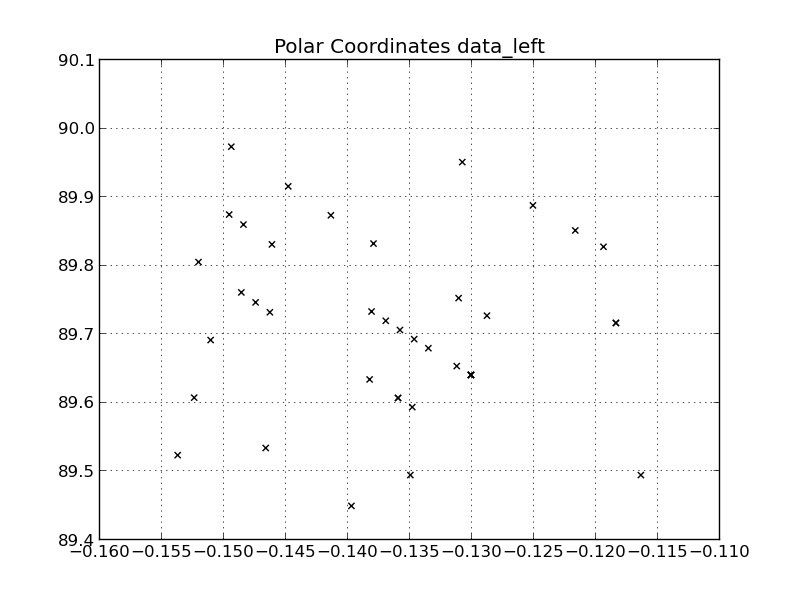
\includegraphics[width=0.5\linewidth]{img/data_left_pc.png}
  %\caption{}
  %\label{fig:}
\end{figure}

\subsubsection{ahead}
\begin{figure}[H]
  \centering
  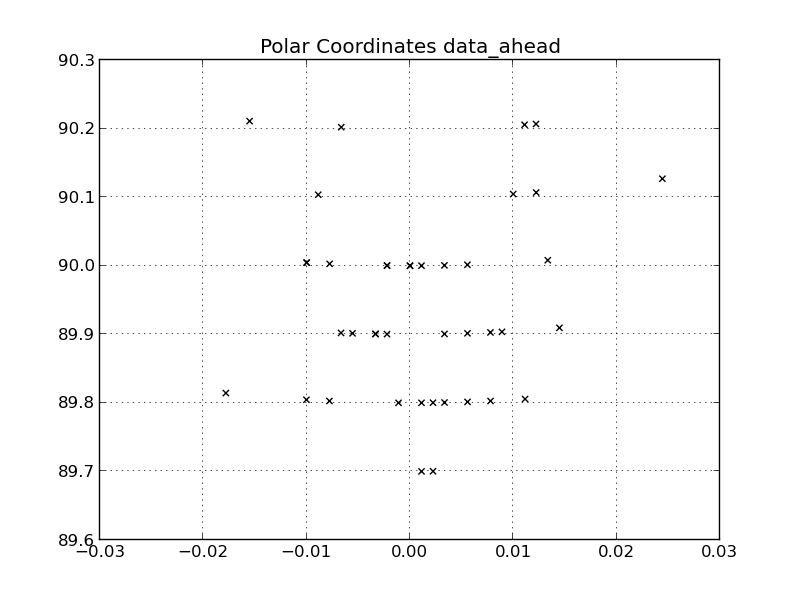
\includegraphics[width=0.5\linewidth]{img/data_ahead_pc.png}
  %\caption{}
  %\label{fig:}
\end{figure}

\subsubsection{right}
\begin{figure}[H]
  \centering
  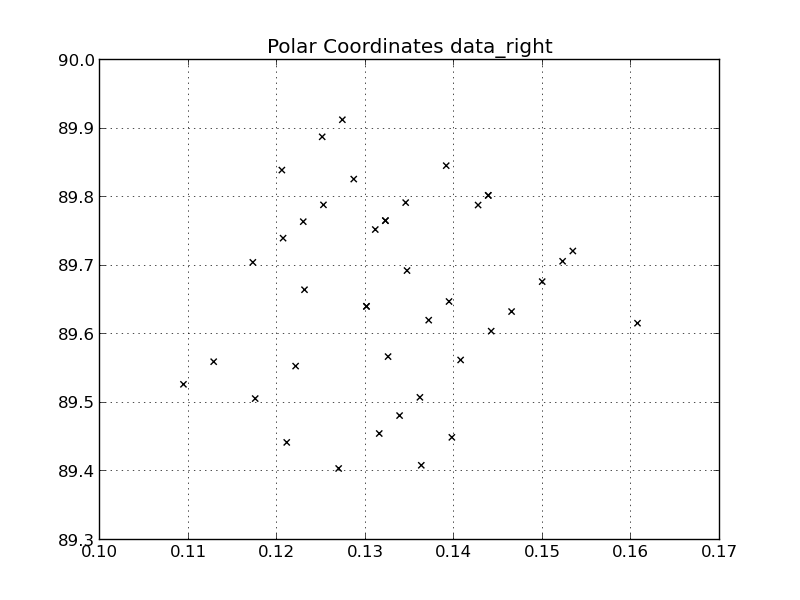
\includegraphics[width=0.5\linewidth]{img/data_right_pc.png}
  %\caption{}
  %\label{fig:}
\end{figure}


\subsection{Boxplots}

\subsection{Angle}

\begin{figure}[H]
  \centering
  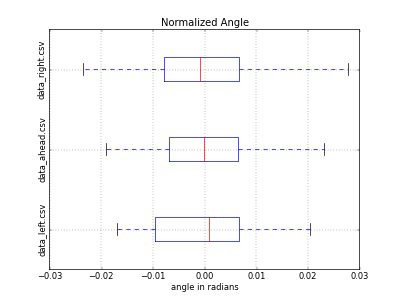
\includegraphics[width=0.5\linewidth]{img/BoxplotAngleNorm.png}
  %\caption{}
  %\label{fig:}
\end{figure}
%Description

\subsection{Distance}
\begin{figure}[H]
  \centering
  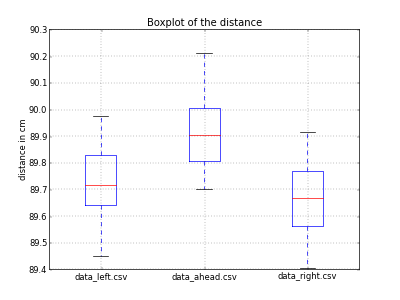
\includegraphics[width=0.5\linewidth]{img/BoxplotDistance.png}
  %\caption{}
  %\label{fig:}
\end{figure}
%Description

\subsection{Distributions}

\subsubsection{left}
\begin{figure}[H]
\centering
\begin{minipage}{.5\textwidth}
  \centering
  \includegraphics[width=1.0\linewidth]{img/Angles_data_left.png}
  %\caption{}
  %\label{fig:}
\end{minipage}%
\begin{minipage}{.5\textwidth}
  \centering
  \includegraphics[width=1.0\linewidth]{img/Distances_data_left.png}
  %\caption{}
  %\label{fig:}
\end{minipage}
\end{figure}
%Description


\subsubsection{ahead}
\begin{figure}[H]
\centering
\begin{minipage}{.5\textwidth}
  \centering
  \includegraphics[width=1.0\linewidth]{img/Angles_data_ahead.png}
  %\caption{}
  %\label{fig:}
\end{minipage}%
\begin{minipage}{.5\textwidth}
  \centering
  \includegraphics[width=1.0\linewidth]{img/Distances_data_ahead.png}
  %\caption{}
  %\label{fig:}
\end{minipage}
\end{figure}

%Description

\subsubsection{right}

\begin{figure}[H]
\centering
\begin{minipage}{.5\textwidth}
  \centering
  \includegraphics[width=1.0\linewidth]{img/Angles_data_right.png}
  %\caption{}
  %\label{fig:}
\end{minipage}%
\begin{minipage}{.5\textwidth}
  \centering
  \includegraphics[width=1.0\linewidth]{img/Distances_data_right.png}
  %\caption{}
  %\label{fig:}
\end{minipage}
\end{figure}

%Description


%CONTENTS
%NOTES


%COPY AND PASTE FROM HERE

%\begin{enumerate}
% \item
%\end{enumerate}

%\href{link}{text}

%\begin[Language=Python]{lstlisting}
%#PYTHON CODE HERE
%\end{lstlisting}

%\lstinputlisting[language=Java]{ }

%\csvautotabular[separator=semicolon]{data.csv}

%\begin{figure}
% \center
% \includegraphics[width= cm]{img/ }
% \caption{}
%\end{figure}

%BIBLIOGRPAHY?
%\bibliographystyle{plain}%amsalpha
%\bibliography{Top30.bib}
%\bibentry{}

\end{document}
